\section{Study case: experiments and evaluation}
To evaluate our system we need some initial data to define the \textit{relevances} (see section \ref{section:context-awareness}) and some (real or simulated) users to test with.

\subsection{Relevances}
To define each $r_{c,x}$ for each node $c$ and context factor $x$, it was decided to gather real data provided by real people through a survey and then average them. The survey consisted of the question "Answer how much a 'context factor' influences your decision to go to a place/event of the specified type (these types are not exclusive)". Then, for each of the ontology classes specified on section \ref{section:context_factors} people had to answer a real value between $0$ and $10$, where:
\begin{itemize}
    \item $0$ means that if the context factor is met, you would not go to the place / event.
    \item 5 means you don't care if the context is met or not.
    \item 10 means that if the context is met, you would go to the place / event.
\end{itemize}

Then the following formula is applied to each feature or column, hence average them and transforming them to be on range $[0,2]$:
$$AVG(column)/5$$

The form had a total of 34 answers. Something worth to mention was that the answers were concentrated between the options $0$, $5$ and $10$, maybe because it is easier to think something between the thoughts "I would not", "I don't care" and "I would", than to think something that is in the middle of two of those thoughts.

\subsection{Users data}
As explained before (see section \ref{section:preferences-propagation}), a user of the system have to give initial preferences to some ontology classes. It was decided to make a form where people could answer their preferences of the higher level ontology classes mentioned before (see section \ref{section:context_factors}). The form had a total of 63 answers. The genre, country, profession, age and (optional) social networks were also asked to have more information for further work. The answer should be integers on range $[1, 10]$. Again, answers were more concentrated on the middle and highest options, but there were few low answers.

\subsubsection{Simulated scenarios}
To evaluate the system, it was decided to test it with simulated scenarios (simulated context and simulated user). A set of clusters were chosen as the set of simulated users. The \textit{K-Means} algorithm was used to get the clusters and the \textit{Elbow Method} (see figure \ref{fig:elbow}) was used to chose $4$ as the number of clusters.
\begin{figure}[h]
    \centering
    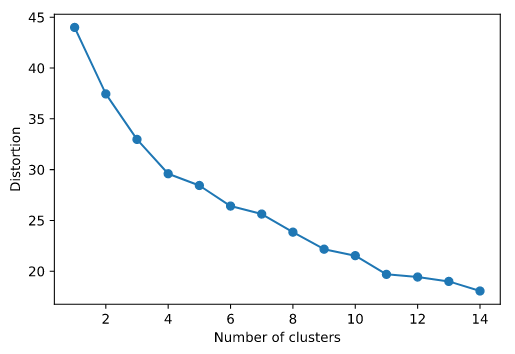
\includegraphics[scale=0.45]{elbow.png}
    \caption{Distortions of the different number of clusters}
    \label{fig:elbow}
\end{figure}

\subsection{Experiments}
For each centroid of the clusters mentioned previously, we simulate two visits to each possible scenario using each possible value for each context factor. The system returns a set of not more than $5$ recommended places inside a radius of $8$ kilometers for each visit. For each recommended set we analyze the average preference, average activation, average aging, average novelty \cite{kotkov2016survey} and average \textit{distance}. To compute novelty we use the metric mentioned on section \ref{section:serendipity}, which is adapted as follow:
\begin{equation} \label{eq:novelty}
    nov(p, u) = \  \underaccent{q \in rec(u)}{min} \  ( dist( c_p, c_q ) )
\end{equation}
where $p$ is a recommended place, $u$ the user to which $p$ was recommended, $rec(u)$ is the set of already recommended places to $u$, $c_p$ is the ontology class to which $p$ belongs and $dist$ computes the distance in the ontology (using \textit{Breadth First Search}) of two ontology classes.